\documentclass{article}	

\usepackage{tikz}
\tikzset{near start abs/.style={xshift=1cm}}
\usetikzlibrary{calc}
\usetikzlibrary{intersections}
\usetikzlibrary{arrows.meta,quotes}
\usepackage{pgfplots}
\usetikzlibrary {datavisualization.formats.functions}
\usetikzlibrary{arrows,scopes}


\usepackage{siunitx}
\usepackage[font=small,labelfont=bf]{caption}
\usepackage{graphicx}
\usepackage{subcaption}
\usepackage{float}

\begin{document}

\begin{figure}[H]
\begin{center}

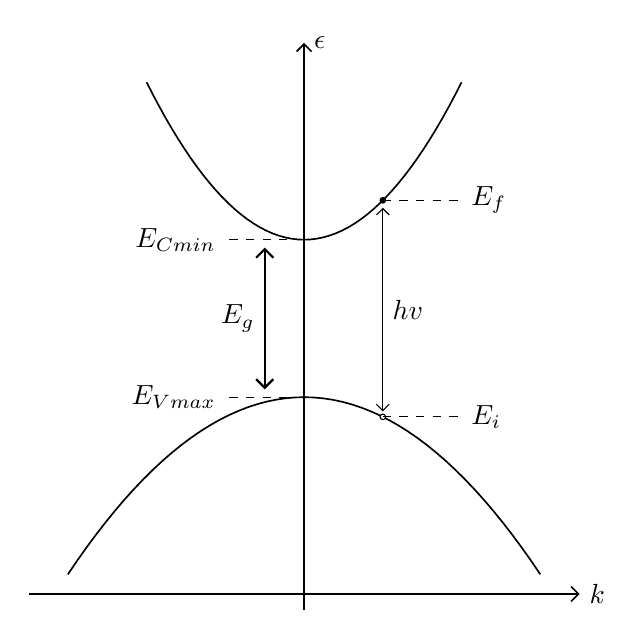
\begin{tikzpicture}[auto, > = Straight Barb, samples = 51]
	\draw[<-,semithick] (0,3.5) -- (0,-3.7) node[anchor=west, pos=0] {$\epsilon$} ; % y axis
	\draw[->, semithick] (-3.5,-3.5) -- (3.5,-3.5) node[anchor=west, pos=1] {$k$} ; % x axis
	
	\draw[-, semithick]   plot [domain=-2:2] (\x, {+1+0.5*(\x)^2});
	\draw[-, semithick]   plot [domain=-3:3] (\x, {-1-0.25*(\x)^2}); 
	
	\draw [fill=white] (1,{-1-0.25*(1)^2}) circle (1pt);
	\draw [fill=black] (1,{+1+0.5*(1)^2}) circle (1pt);
	
	\draw[dashed] (0,1) -- (-1,1) node[anchor=east] {$E_{Cmin}$};
	\draw[dashed] (0,-1) -- (-1,-1) node[anchor=east] {$E_{Vmax}$};
	\draw[<->, thick] (-0.5,-0.9) -- (-0.5,0.9) node[anchor=east, midway] {$E_{g}$};
	\draw[dashed] (1,{+1+0.5*(1)^2}) -- (2,{+1+0.5*(1)^2}) node[anchor=west] {$E_{f}$};
	\draw[dashed] (1,{-1-0.25*(1)^2}) -- (2,{-1-0.25*(1)^2}) node[anchor=west] {$E_{i}$};
	
	\draw (1,{-1-0.25*(0.85)^2}) coordinate (p1) node[]{};
	\draw (1,{+1+0.5*(0.9)^2}) coordinate (p2) node[]{};
	%\draw[<->]  (1,{-1-0.25*(0.9)^2}) to ["{1}"]((1,{1+0.5*(0.9)^2});
	\draw[<->]  (p1) -- (p2) node[anchor=west, midway]{$hv$};
\end{tikzpicture}

\caption{\label{fig:DirectBandgap}Direct Bandgap Complete}
\end{center}

\end{figure}

\begin{figure}[h]
\begin{center}

\begin{tikzpicture}[auto, > = Straight Barb, samples = 51,
declare function={ conduction(\x) = +1+0.75*(\x - 3)^2;
				   valence(\x)    = -1-0.25*(\x)^2;
				  },]

	\draw[<-,semithick] (0,3.5) -- (0,-3.7) node[anchor=west, pos=0] {$\epsilon$} ; % y axis
	\draw[->, semithick] (-3.5,-3.5) -- (5,-3.5) node[anchor=west, pos=1] {$k$} ; % x axis
	
	\draw[-, semithick]   plot [domain=1.2:4.8] (\x, {conduction(\x)});
	\draw[-, semithick]   plot [domain=-3:3] (\x, {valence{\x}}); 
	
	\draw [fill=black] (3,{conduction(3)}) circle (2pt);
	\draw [fill=white] (1,{valence(1)}) circle (2pt);
	
	\draw[dashed] (0,1) -- (-1,1) node[anchor=east] {$E_{Cmin}$};
	\draw[dashed] (0,-1) -- (-1,-1) node[anchor=east] {$E_{Vmax}$};
	\draw[<->, thick] (-0.5,-0.9) -- (-0.5,0.9) node[anchor=east, midway] {$E_{g}$};
	
	\draw[dashed, shorten <=5pt] (3,{conduction(3)}) -- (4,{conduction(3)}) node[anchor=west] {$E_{f}$};
	\draw[dashed, shorten <=5pt] (1,{valence(1)}) -- (2,{valence(1)}) node[anchor=west] {$E_{i}$};
	
	\draw (1,{conduction(0.9)}) coordinate (p1) node[]{};
	\draw (1,{valence(0.85)}) coordinate (p2) node[]{};
	
	\draw[->,thick, shorten <=3pt, shorten >=1pt] (1,{valence(1)}) -- (1, 0.5) node [midway, above, sloped] (photon-node) {photon};
	\draw[->,thick, shorten <=1pt, shorten >=3pt] (1, 0.5) -- (2.9, {conduction(3)}) node [midway, below, sloped] (phonon-e-node) {photon};

\end{tikzpicture}

\caption{\label{fig:IndirectPhononAbsorption} Indirect Bandgap Phonon Absorption}
\end{center}

\end{figure}


\begin{figure}[h]
\begin{center}

\begin{tikzpicture}[auto, > = Straight Barb, samples = 51,
declare function={ conduction(\x) = +1+0.75*(\x - 3)^2;
				   valence(\x)    = -1-0.25*(\x)^2;
				  },]

	\draw[<-,semithick] (0,3.5) -- (0,-3.7) node[anchor=west, pos=0] {$\epsilon$} ; % y axis
	\draw[->, semithick] (-3.5,-3.5) -- (5,-3.5) node[anchor=west, pos=1] {$k$} ; % x axis
	
	\draw[-, semithick]   plot [domain=1.2:4.8] (\x, {conduction(\x)});
	\draw[-, semithick]   plot [domain=-3:3] (\x, {valence{\x}}); 
	
	\draw [fill=black] (3,{conduction(3)}) circle (2pt);
	\draw [fill=white] (1,{valence(1)}) circle (2pt);
	
	\draw[dashed] (0,1) -- (-1,1) node[anchor=east] {$E_{Cmin}$};
	\draw[dashed] (0,-1) -- (-1,-1) node[anchor=east] {$E_{Vmax}$};
	\draw[<->, thick] (-0.5,-0.9) -- (-0.5,0.9) node[anchor=east, midway] {$E_{g}$};
	
	\draw[dashed] (3,{conduction(3)}) -- (4,{conduction(3)}) node[anchor=west] {$E_{f}$};
	\draw[dashed] (1,{valence(1)}) -- (2,{valence(1)}) node[anchor=west] {$E_{i}$};
	
	\draw (1,{conduction(0.9)}) coordinate (p1) node[]{};
	\draw (1,{valence(0.85)}) coordinate (p2) node[]{};
	
	\draw[->,thick, shorten <=3pt, shorten >=3pt] (1,{valence(1)}) -- (1, 2.5) node [midway, above, sloped] (photon-node) {photon};
	\draw[->,thick, shorten <=3pt, shorten >=1pt] (1, 2.5) -- (2.9, {conduction(3.3)}) node [midway, below, sloped] (phonon-a-node) {phonon};

\end{tikzpicture}

\caption{\label{fig:IndirectPhononAbsorption} Indirect Bandgap Phonon Absorption}
\end{center}

\end{figure}

\begin{figure}[h]
\begin{center}

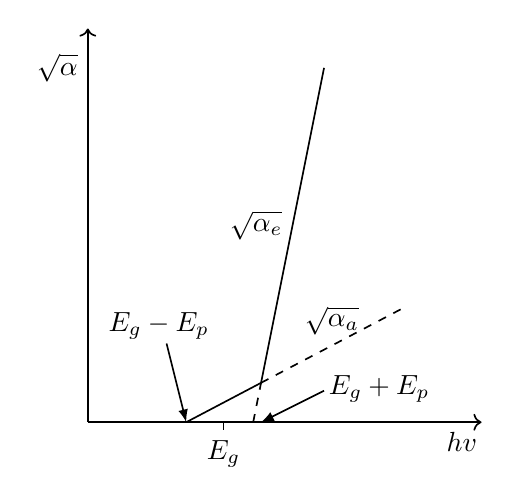
\begin{tikzpicture}
  \node (a) at (1.25,-5) {};
  \node (b) at (2.2,-4.5) {};
  \node (c) at (3,-0.5) {};


\draw[->,semithick] (0,-5) -- (0,0) node[anchor=east, pos=0.9] {$\sqrt{\alpha}$} ; % y axis
\draw[->, semithick] (0,-5) -- (5,-5) node[anchor=north, pos=0.95] {$hv$} ; % x axis

\draw[-,semithick, line cap=round] (1.25,-5) -- (2.2,-4.5) node[anchor=east, pos=0.5] {$$} ;
\draw[-,semithick] (2.2,-4.5) -- (3,-0.5) node[anchor=east, pos=0.5] {$\sqrt{\alpha_e}$} ; 
\draw[dashed,semithick] (2.1,-5) -- (2.2,-4.5) node[anchor=east, pos=0.5] {$$} ; 
\draw[dashed,semithick] (2.2,-4.5) -- (4,-3.55263157895) node[anchor=south, pos=0.5] {$\sqrt{\alpha_a}$} ; 

%\draw[-,semithick] (1.25,-5) -- (1.25,-5.1) node[anchor=east, pos=0.5] {$$} ; 
\draw[-,semithick] (1.725,-5) -- (1.725,-5.1) node[anchor=north, pos=1] {$E_g$} ; 
%\draw[-,semithick] (2.1,-5) -- (2.1,-5.1) node[anchor=east, pos=0.5] {$$} ; 

\draw[->,semithick, ball/.style={ellipse, minimum width=3cm, minimum height=1.5cm, draw},>=latex] (1,-4) -- (1.25,-5) node[label={[xshift=-0.35cm, yshift=0.8cm]$E_g-E_p$}] {} ; % y axis
\draw[->,semithick, ball/.style={ellipse, minimum width=3cm, minimum height=1.5cm, draw},>=latex] (3,-4.6) -- (2.2,-5) node[label={[xshift=1.5cm, yshift=0cm]$E_g+E_p$}] {} ; % y axis


\end{tikzpicture}

\caption{\label{fig:} Axis}
\end{center}

\end{figure}

\begin{figure}[]
\begin{center}

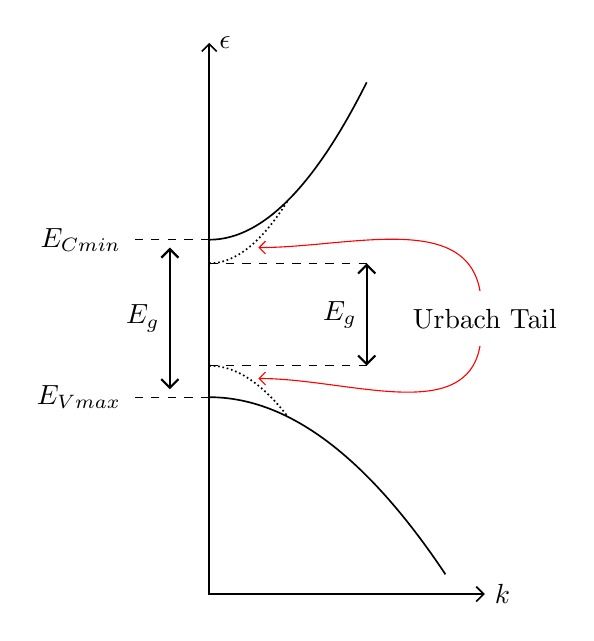
\begin{tikzpicture}[auto, > = Straight Barb, samples = 51]
	\draw[<-,semithick] (0,3.5) -- (0,-3.51) node[anchor=west, pos=0] {$\epsilon$} ; % y axis
	\draw[->, semithick] (0,-3.5) -- (3.5,-3.5) node[anchor=west, pos=1] {$k$} ; % x axis
	
	\draw[-, semithick]   plot [domain=0:2] (\x, {+1+0.5*(\x)^2});
	\draw[-, semithick]   plot [domain=0:3] (\x, {-1-0.25*(\x)^2}); 
	
	\draw[densely dotted, semithick]   plot [domain=0:1] (\x, {-0.6-0.65*(\x)^2});
	\draw[densely dotted, semithick]   plot [domain=0:1] (\x, {+0.7+0.8*(\x)^2});

	
	\draw[dashed] (0,1) -- (-1,1) node[anchor=east] {$E_{Cmin}$};
	\draw[dashed] (0,-1) -- (-1,-1) node[anchor=east] {$E_{Vmax}$};
	\draw[<->, thick] (-0.5,-0.9) -- (-0.5,0.9) node[anchor=east, midway] {$E_{g}$};
	
	\draw[dashed] (0,{-0.6-0.65*(0)^2}) -- (2,{-0.6-0.65*(0)^2}) node[anchor=west] {$$};
	\draw[dashed] (0,{+0.7+0.8*(0)^2}) -- (2,{+0.7+0.8*(0)^2}) node[anchor=west] {$$};
	\draw[<->, thick] (2,{+0.7+0.8*(0)^2}) -- (2,{-0.6-0.65*(0)^2}) node[anchor=east, midway] {$E_{g}$};
	
	\node (a) at (0.5,{-0.6-0.65*(0.5)^2}) {};
	\node (b) at (0.5,{+0.7+0.8*(0.5)^2}) {};
	\node (c) at (2.5,0) {};
	\node (c) at (3.5,0) {Urbach Tail};

	
	\path [red,,->, out=260,in=0, shorten <=3pt] (c) edge (a);
	\path [red,,->, out=-260,in=0, shorten <=3pt] (c) edge (b);
	
	\draw (1,{-1-0.25*(0.85)^2}) coordinate (p1) node[]{};
	\draw (1,{+1+0.5*(0.9)^2}) coordinate (p2) node[]{};
	%\draw[<->]  (1,{-1-0.25*(0.9)^2}) to ["{1}"]((1,{1+0.5*(0.9)^2});
	%\draw[<->]  (p1) -- (p2) node[anchor=west, midway]{$hv$};
\end{tikzpicture}

\caption{\label{fig:DirectBandgap}Urbach Tail}
\end{center}

\end{figure}

\end{document}
